\documentclass{beamer}
\usepackage[utf8]{inputenc}

\usetheme{Madrid}
\usecolortheme{default}
\usepackage{amsmath,amssymb,amsfonts,amsthm}
\usepackage{txfonts}
\usepackage{tkz-euclide}
\usepackage{listings}
\usepackage{adjustbox}
\usepackage{array}
\usepackage{tabularx}
\usepackage{gvv}
\usepackage{lmodern}
\usepackage{circuitikz}
\usepackage{tikz}
\usepackage{graphicx}
\usepackage[T1]{fontenc}
\usepackage[utf8]{inputenc}

\lstset{
  language=Python,
  basicstyle=\ttfamily\small,
  breaklines=true,
  literate={λ}{{$\lambda$}}1
}



\setbeamertemplate{page number in head/foot}[totalframenumber]

\usepackage{tcolorbox}
\tcbuselibrary{minted,breakable,xparse,skins}



\definecolor{bg}{gray}{0.95}
\DeclareTCBListing{mintedbox}{O{}m!O{}}{%
  breakable=true,
  listing engine=minted,
  listing only,
  minted language=#2,
  minted style=default,
  minted options={%
    linenos,
    gobble=0,
    breaklines=true,
    breakafter=,,
    fontsize=\small,
    numbersep=8pt,
    #1},
  boxsep=0pt,
  left skip=0pt,
  right skip=0pt,
  left=25pt,
  right=0pt,
  top=3pt,
  bottom=3pt,
  arc=5pt,
  leftrule=0pt,
  rightrule=0pt,
  bottomrule=2pt,
  toprule=2pt,
  colback=bg,
  colframe=orange!70,
  enhanced,
  overlay={%
    \begin{tcbclipinterior}
    \fill[orange!20!white] (frame.south west) rectangle ([xshift=20pt]frame.north west);
    \end{tcbclipinterior}},
  #3,
}
\lstset{
    language=C,
    basicstyle=\ttfamily\small,
    keywordstyle=\color{blue},
    stringstyle=\color{orange},
    commentstyle=\color{green!60!black},
    numbers=left,
    numberstyle=\tiny\color{gray},
    breaklines=true,
    showstringspaces=false,
}
\begin{document}

\title 
{4.10.17}
\date{September 14,2025}


\author 
{Bhoomika V - EE25BTECH11015}




\frame{\titlepage}
\begin{frame}{Question}
Compute the area bounded by the lines $x + 2y = 2$, $y - x = 1$, and $2x + y = 7$.
\end{frame}

\begin{frame}{equations of the line}

\[
L_1: x + 2y = 2, \quad 
L_2: y - x = 1, \quad
L_3: 2x + y = 7
\]


 Finding intersection points using RREF \\
\end{frame}  

\begin{frame}{Point A}
Intersection of $L_1$ and $L_2$:
\[
\begin{cases}
x + 2y = 2 \\
-x + y = 1
\end{cases}
\]
\[
\left[\begin{array}{cc|c}
1 & 2 & 2 \\
-1 & 1 & 1
\end{array}\right]
\;\;\xrightarrow{\text{RREF}}\;\;
\left[\begin{array}{cc|c}
1 & 0 & 0 \\
0 & 1 & 1
\end{array}\right]
\]
\[
A= (0,1)
\]
\end{frame}

\begin{frame}{Point B}
Intersection of $L_2$ and $L_3$:
\[
\begin{cases}
-x + y = 1 \\
2x + y = 7
\end{cases}
\]
\[
\left[\begin{array}{cc|c}
-1 & 1 & 1 \\
2 & 1 & 7
\end{array}\right]
\;\;\xrightarrow{\text{RREF}}\;\;
\left[\begin{array}{cc|c}
1 & 0 & 2 \\
0 & 1 & 3
\end{array}\right]
\]
\[
B = (2,3)
\]
\end{frame}

\begin{frame}{Point C}
Intersection of $L_1$ and $L_3$:
\[
\begin{cases}
x + 2y = 2 \\
2x + y = 7
\end{cases}
\]
\[
\left[\begin{array}{cc|c}
1 & 2 & 2 \\
2 & 1 & 7
\end{array}\right]
\;\;\xrightarrow{\text{RREF}}\;\;
\left[\begin{array}{cc|c}
1 & 0 & 4 \\
0 & 1 & -1
\end{array}\right]
\]
\[
C = (4,-1)
\]
\end{frame}

\begin{frame}{Area}
Area of the triangle

\[
\Delta = \tfrac{1}{2} \left| (\vec{A}-\vec{B}) \times (\vec{B}-\vec{C}) \right|
\]

Compute:
\[
\vec{A} - \vec{B} = \begin{bmatrix} -2 \\ -2 \end{bmatrix}, \quad
\vec{B} - \vec{C} = \begin{bmatrix} -2 \\ 4 \end{bmatrix}
\]

\[
(\vec{A}-\vec{B}) \times (\vec{B}-\vec{C}) =
\begin{vmatrix}
-2 & -2 \\
-2 & 4
\end{vmatrix}
= (-2)(4) - (-2)(-2) = -12
\]

\[
\Delta = \tfrac{1}{2} | -12 | = 6
\]
\end{frame}

\begin{frame}[fragile]
    \begin{lstlisting}
#include <math.h>

// Function to compute area of a triangle given 3 points (x,y,z)
float triangle_area(float x1, float y1, float z1,
                    float x2, float y2, float z2,
                    float x3, float y3, float z3) {

    // Using cross product method: Area = 0.5 * |AB x AC|
    float ABx = x2 - x1;
    float ABy = y2 - y1;
    float ABz = z2 - z1;

    float ACx = x3 - x1;
    float ACy = y3 - y1;
    float ACz = z3 - z1;
     \end{lstlisting}
\end{frame}

\begin{frame}[fragile]
    \begin{lstlisting}

    // Cross product AB x AC
    float cross_x = ABy*ACz - ABz*ACy;
    float cross_y = ABz*ACx - ABx*ACz;
    float cross_z = ABx*ACy - ABy*ACx;

    // Magnitude of cross product
    float area = 0.5 * sqrt(cross_x*cross_x + cross_y*cross_y + cross_z*cross_z);
    return area;
}

     \end{lstlisting}
\end{frame}

\begin{frame}[fragile]
    \frametitle{Python Code}
    \begin{lstlisting}
import numpy as np
import matplotlib.pyplot as plt
import ctypes
import os

# --- Load the C library ---
try:
    c_lib = ctypes.CDLL('./code.so')
except OSError:
    print("Error: 'code.so' not found. Compile using: gcc -shared -o code.so -fPIC triangle.c -lm")
    exit()
    \end{lstlisting}
\end{frame}

\begin{frame}[fragile]
    \frametitle{Python Code}
    \begin{lstlisting}
# Define argument and return types
c_lib.triangle_area.argtypes = [ctypes.c_float, ctypes.c_float, ctypes.c_float,
                                ctypes.c_float, ctypes.c_float, ctypes.c_float,
                                ctypes.c_float, ctypes.c_float, ctypes.c_float]
c_lib.triangle_area.restype = ctypes.c_float

# --- Triangle vertices (intersection points of the lines) ---
A = np.array([0, 1, 0], dtype=np.float32)     # x+2y=2 & y-x=1
B = np.array([2, 3, 0], dtype=np.float32)     # y-x=1 & 2x+y=7
C = np.array([3, -0.5, 0], dtype=np.float32)  # x+2y=2 & 2x+y=7

# --- Call C function ---
area = c_lib.triangle_area(A[0], A[1], A[2],
                           B[0], B[1], B[2],
                           C[0], C[1], C[2])
print(f"Area of triangle = {area:.2f}")

    \end{lstlisting}
\end{frame}

\begin{frame}[fragile]
    \frametitle{Python Code}
    \begin{lstlisting}
# --- Plotting ---
fig, ax = plt.subplots(figsize=(6,6))

# Triangle edges
ax.plot([A[0], B[0]], [A[1], B[1]], color="black")
ax.plot([B[0], C[0]], [B[1], C[1]], color="black")
ax.plot([C[0], A[0]], [C[1], A[1]], color="black")

# Fill triangle
ax.fill([A[0], B[0], C[0]], [A[1], B[1], C[1]], color="cyan", alpha=0.3)
# Points
ax.scatter(A[0], A[1], color="red", s=60)
ax.scatter(B[0], B[1], color="blue", s=60)
ax.scatter(C[0], C[1], color="green", s=60)

    \end{lstlisting}
\end{frame}

\begin{frame}[fragile]
    \frametitle{Python Code}
    \begin{lstlisting}

# Labels
ax.text(A[0]+0.1, A[1], "A(0,1)", color="red")
ax.text(B[0]+0.1, B[1], "B(2,3)", color="blue")
ax.text(C[0]+0.1, C[1], "C(3,-0.5)", color="green")

# Area annotation
ax.text(1.5, 1.5, f"Area = {area:.2f}", color="purple", fontsize=12)

# Formatting
ax.set_xlabel("X-axis")
ax.set_ylabel("Y-axis")
ax.set_title("Triangle formed by intersection of lines")
ax.grid(True)
ax.set_aspect("equal")

plt.show()


    \end{lstlisting}
\end{frame}

\begin{frame}{Plot}
    \centering
    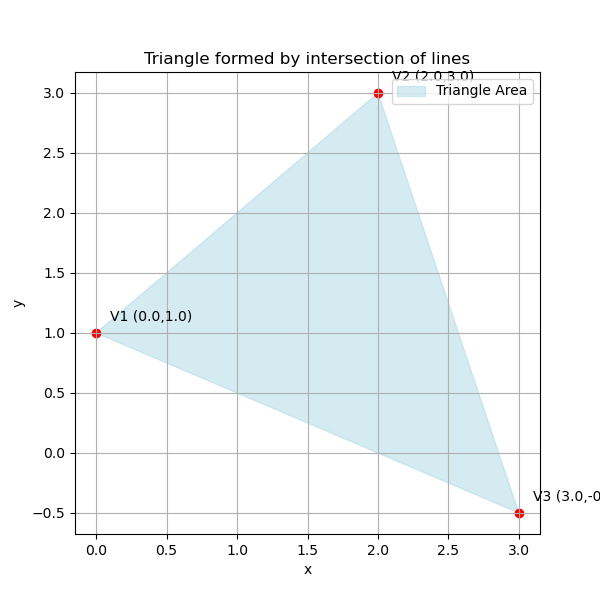
\includegraphics[width=\columnwidth, height=0.8\textheight, keepaspectratio]{Figs/Fig1.png}     
\end{frame}



\end{document}